\documentclass{homework}

\title{Example title: Linear Algebra}
\author{T. Fitzgerald}
\date{3 January 2024}
\addbibresource{refs.bib}

\begin{document}

\maketitle
\tableofcontents
% \newpage

%-------------------------------------------------------------
\section{Problem 1}

\subsection{Part 1}
We can make a citation directly, such as \citet{Udwadia2007}.
Or we can make a parenthetical reference \citep{Ackermann1972}.
Making a list of references also works \citep{Willard2018,Akhtaruzzaman2010,Trefethen2015}.
To make a reference to an equation we can use \texttt{label} and \texttt{eqref} to get \eqref{eq:num1}.

\begin{align}\label{eq:num1}
    \Ten{I}_O = \int\limits_\Omega \rho \left( |\Vec{r}|_2 \Ten{E}_3 - \Vec{r} \otimes \Vec{r}  \right) \diff V
\end{align}

Common environments to use are \texttt{align}, \texttt{gather}, and \texttt{multline}.
\begin{align}
    a_0 &= \frac{1}{T}\int\limits_{-T/2}^{T/2} f(t)\diff t
    \\
    a_n &= \frac{2}{T} \int\limits_{-T/2}^{T/2} f(t) \cos(n \omega_0 t)\diff t
    \\
    b_n &= \frac{2}{T} \int\limits_{-T/2}^{T/2} f(t) \sin(n \omega_0 t)\diff t \, .
\end{align}
  

%-------------------------------------------------------------
\newpage
\section{Problem 2}

Including a figure is straightforward using the following pattern.
Referencing the figure with a \texttt{ref}, such as Fig \ref{fig:cam:accel}.
Be sure to replace \texttt{examplefig} with the filename of the image you want to include.

\begin{figure}[h!]
    \centering
    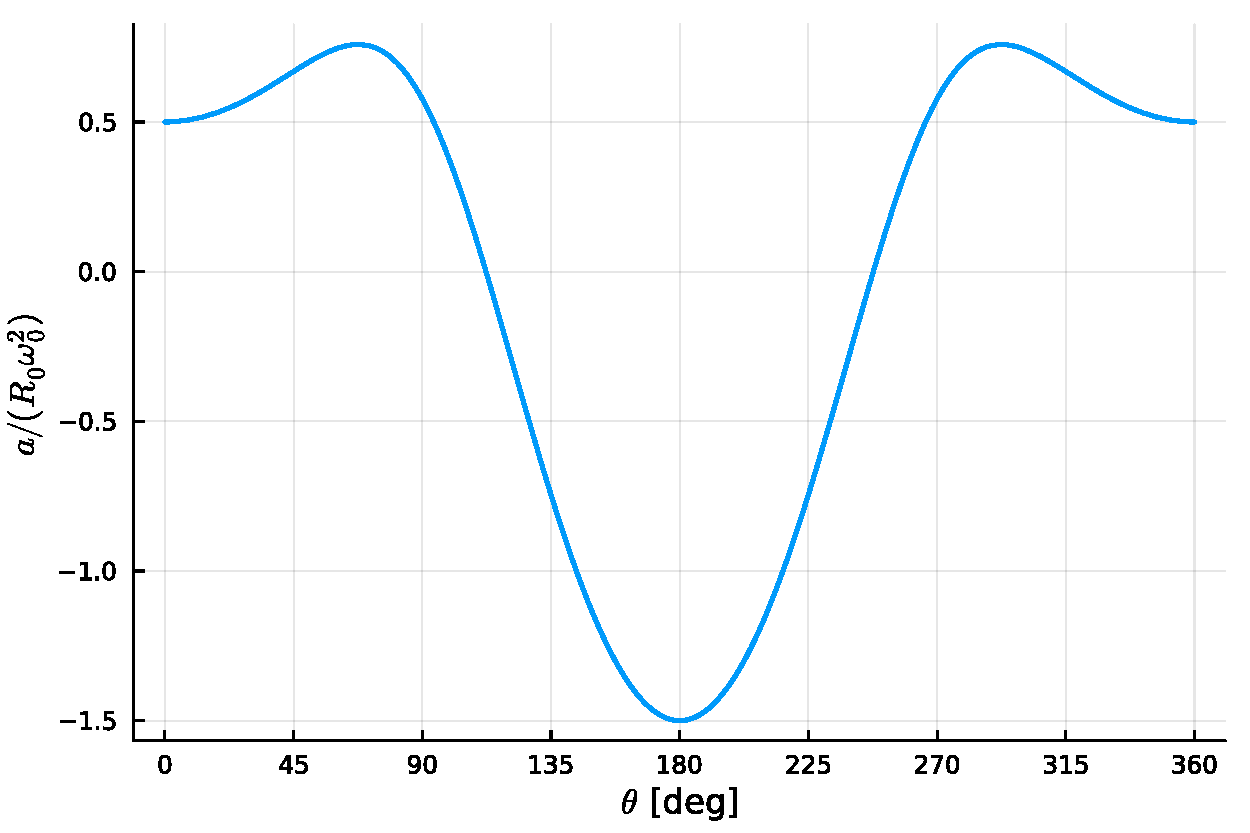
\includegraphics[width=4in]{examplefig}
    \caption{Cam acceleration as a function of angle $\theta$ normalized by $R_0 = R(\theta\to 0) = 3\text{ in}$.}
    \label{fig:cam:accel}
\end{figure}

%-------------------------------------------------------------
\newpage
\section{Problem 3}\label{sec:p3}
Referencing the table matches the pattern of a figure using a \texttt{ref}, such as Table \ref{tab:cam}.


\begin{table}[h]
  \caption{Parameter values for \S\ref{sec:p3}}
    \label{tab:cam}
    \begin{center}
      \begin{tabular}{crl}
        \toprule
        \textbf{Quantity} & \multicolumn{2}{c}{\textbf{Value}} \\
        \midrule
        $w$     &  0.5  & lb \\
        $\mu_k$ &  0.2  &  \\
        \bottomrule
      \end{tabular}
  \end{center}
\end{table}


%-------------------------------------------------------------
\newpage
\section{Problem 4}\label{sec:p4}
Including a code snippet is done using the \href{https://www.overleaf.com/learn/latex/Code_listing}{Listings Package}.
There is a custom defined Matlab format in the homework class file, and other languages can also be used.
See the package documentation for more options.
To include an incline snippet using an \texttt{lstlisting} environment

\begin{lstlisting}[language=Matlab]
x = linspace(0, 2, 100);
y = 2*sin(x);
% make a plot
plot(x,y);
\end{lstlisting}

Longer code files are added using an \texttt{lstinputlisting} command 
\lstinputlisting[language=Matlab]{simple.m}



%%%%%%%%%%%%%%%%%%%%%%%%%%%%%%%%%%%%%%%%%%%%%%%
\printbibliography
\end{document}